% Options for packages loaded elsewhere
\PassOptionsToPackage{unicode}{hyperref}
\PassOptionsToPackage{hyphens}{url}
%
\documentclass[
  12pt,
]{article}
\usepackage{amsmath,amssymb}
\usepackage{iftex}
\ifPDFTeX
  \usepackage[T1]{fontenc}
  \usepackage[utf8]{inputenc}
  \usepackage{textcomp} % provide euro and other symbols
\else % if luatex or xetex
  \usepackage{unicode-math} % this also loads fontspec
  \defaultfontfeatures{Scale=MatchLowercase}
  \defaultfontfeatures[\rmfamily]{Ligatures=TeX,Scale=1}
\fi
\usepackage{lmodern}
\ifPDFTeX\else
  % xetex/luatex font selection
\fi
% Use upquote if available, for straight quotes in verbatim environments
\IfFileExists{upquote.sty}{\usepackage{upquote}}{}
\IfFileExists{microtype.sty}{% use microtype if available
  \usepackage[]{microtype}
  \UseMicrotypeSet[protrusion]{basicmath} % disable protrusion for tt fonts
}{}
\makeatletter
\@ifundefined{KOMAClassName}{% if non-KOMA class
  \IfFileExists{parskip.sty}{%
    \usepackage{parskip}
  }{% else
    \setlength{\parindent}{0pt}
    \setlength{\parskip}{6pt plus 2pt minus 1pt}}
}{% if KOMA class
  \KOMAoptions{parskip=half}}
\makeatother
\usepackage{xcolor}
\usepackage[margin=1in]{geometry}
\usepackage{color}
\usepackage{fancyvrb}
\newcommand{\VerbBar}{|}
\newcommand{\VERB}{\Verb[commandchars=\\\{\}]}
\DefineVerbatimEnvironment{Highlighting}{Verbatim}{commandchars=\\\{\}}
% Add ',fontsize=\small' for more characters per line
\usepackage{framed}
\definecolor{shadecolor}{RGB}{248,248,248}
\newenvironment{Shaded}{\begin{snugshade}}{\end{snugshade}}
\newcommand{\AlertTok}[1]{\textcolor[rgb]{0.94,0.16,0.16}{#1}}
\newcommand{\AnnotationTok}[1]{\textcolor[rgb]{0.56,0.35,0.01}{\textbf{\textit{#1}}}}
\newcommand{\AttributeTok}[1]{\textcolor[rgb]{0.13,0.29,0.53}{#1}}
\newcommand{\BaseNTok}[1]{\textcolor[rgb]{0.00,0.00,0.81}{#1}}
\newcommand{\BuiltInTok}[1]{#1}
\newcommand{\CharTok}[1]{\textcolor[rgb]{0.31,0.60,0.02}{#1}}
\newcommand{\CommentTok}[1]{\textcolor[rgb]{0.56,0.35,0.01}{\textit{#1}}}
\newcommand{\CommentVarTok}[1]{\textcolor[rgb]{0.56,0.35,0.01}{\textbf{\textit{#1}}}}
\newcommand{\ConstantTok}[1]{\textcolor[rgb]{0.56,0.35,0.01}{#1}}
\newcommand{\ControlFlowTok}[1]{\textcolor[rgb]{0.13,0.29,0.53}{\textbf{#1}}}
\newcommand{\DataTypeTok}[1]{\textcolor[rgb]{0.13,0.29,0.53}{#1}}
\newcommand{\DecValTok}[1]{\textcolor[rgb]{0.00,0.00,0.81}{#1}}
\newcommand{\DocumentationTok}[1]{\textcolor[rgb]{0.56,0.35,0.01}{\textbf{\textit{#1}}}}
\newcommand{\ErrorTok}[1]{\textcolor[rgb]{0.64,0.00,0.00}{\textbf{#1}}}
\newcommand{\ExtensionTok}[1]{#1}
\newcommand{\FloatTok}[1]{\textcolor[rgb]{0.00,0.00,0.81}{#1}}
\newcommand{\FunctionTok}[1]{\textcolor[rgb]{0.13,0.29,0.53}{\textbf{#1}}}
\newcommand{\ImportTok}[1]{#1}
\newcommand{\InformationTok}[1]{\textcolor[rgb]{0.56,0.35,0.01}{\textbf{\textit{#1}}}}
\newcommand{\KeywordTok}[1]{\textcolor[rgb]{0.13,0.29,0.53}{\textbf{#1}}}
\newcommand{\NormalTok}[1]{#1}
\newcommand{\OperatorTok}[1]{\textcolor[rgb]{0.81,0.36,0.00}{\textbf{#1}}}
\newcommand{\OtherTok}[1]{\textcolor[rgb]{0.56,0.35,0.01}{#1}}
\newcommand{\PreprocessorTok}[1]{\textcolor[rgb]{0.56,0.35,0.01}{\textit{#1}}}
\newcommand{\RegionMarkerTok}[1]{#1}
\newcommand{\SpecialCharTok}[1]{\textcolor[rgb]{0.81,0.36,0.00}{\textbf{#1}}}
\newcommand{\SpecialStringTok}[1]{\textcolor[rgb]{0.31,0.60,0.02}{#1}}
\newcommand{\StringTok}[1]{\textcolor[rgb]{0.31,0.60,0.02}{#1}}
\newcommand{\VariableTok}[1]{\textcolor[rgb]{0.00,0.00,0.00}{#1}}
\newcommand{\VerbatimStringTok}[1]{\textcolor[rgb]{0.31,0.60,0.02}{#1}}
\newcommand{\WarningTok}[1]{\textcolor[rgb]{0.56,0.35,0.01}{\textbf{\textit{#1}}}}
\usepackage{graphicx}
\makeatletter
\def\maxwidth{\ifdim\Gin@nat@width>\linewidth\linewidth\else\Gin@nat@width\fi}
\def\maxheight{\ifdim\Gin@nat@height>\textheight\textheight\else\Gin@nat@height\fi}
\makeatother
% Scale images if necessary, so that they will not overflow the page
% margins by default, and it is still possible to overwrite the defaults
% using explicit options in \includegraphics[width, height, ...]{}
\setkeys{Gin}{width=\maxwidth,height=\maxheight,keepaspectratio}
% Set default figure placement to htbp
\makeatletter
\def\fps@figure{htbp}
\makeatother
\setlength{\emergencystretch}{3em} % prevent overfull lines
\providecommand{\tightlist}{%
  \setlength{\itemsep}{0pt}\setlength{\parskip}{0pt}}
\setcounter{secnumdepth}{-\maxdimen} % remove section numbering
\usepackage{graphicx}
\usepackage{fancyhdr}
\usepackage{mdframed}
\pagestyle{fancy}
\fancyhead{}
\fancyhead[L]{\includegraphics[width=3cm]{logo.jpg}}
\fancyhead[R]{\hspace{0.5cm} Universidad Diego Portales \\ Facultad de Administración y Economía}
\fancypagestyle{plain}{ \fancyhead{} \fancyhead[L]{\includegraphics[width=3cm]{logo.jpg}} \fancyhead[R]{\hspace{0.5 cm} Universidad Diego Portales \\ Facultad de Administración y Economía}}
\ifLuaTeX
  \usepackage{selnolig}  % disable illegal ligatures
\fi
\usepackage{bookmark}
\IfFileExists{xurl.sty}{\usepackage{xurl}}{} % add URL line breaks if available
\urlstyle{same}
\hypersetup{
  pdftitle={Ejercicio 3},
  hidelinks,
  pdfcreator={LaTeX via pandoc}}

\title{\textbf{Ejercicio 3}}
\author{}
\date{\vspace{-2.5em}}

\begin{document}
\maketitle

\maketitle
\vspace{-5em}
\vspace{0.5em}

\begin{center}
\footnotesize \textbf{Curso}: Econometría II \\
\footnotesize \textbf{Profesor}: Mauricio Tejada \\
\footnotesize \textbf{Estudiantes}: Dania Bustamante, Rosana Cardona, José Casanova \\
\footnotesize 5 junio 2024 \\
\end{center}

\begin{Shaded}
\begin{Highlighting}[]
\NormalTok{base }\OtherTok{\textless{}{-}} \FunctionTok{read\_excel}\NormalTok{(}\StringTok{"pib\_fbkf\_chile.xlsx"}\NormalTok{, }\AttributeTok{skip =} \DecValTok{2}\NormalTok{)}
\FunctionTok{colnames}\NormalTok{(base) }\OtherTok{\textless{}{-}} \FunctionTok{c}\NormalTok{(}\StringTok{"Periodo"}\NormalTok{, }\StringTok{"fbcf"}\NormalTok{, }\StringTok{"PIB"}\NormalTok{)}
\NormalTok{base}\SpecialCharTok{$}\NormalTok{Periodo }\OtherTok{\textless{}{-}} \FunctionTok{as.Date}\NormalTok{(base}\SpecialCharTok{$}\NormalTok{Periodo, }\AttributeTok{format=}\StringTok{"\%Y{-}\%m{-}\%d"}\NormalTok{)}
\end{Highlighting}
\end{Shaded}

\section{\texorpdfstring{\textbf{\emph{Pregunta
1:}}}{Pregunta 1:}}\label{pregunta-1}

Creación variables logaritmicas y diferencias

\begin{Shaded}
\begin{Highlighting}[]
\CommentTok{\#Var log}
\NormalTok{base }\OtherTok{\textless{}{-}}\NormalTok{ base }\SpecialCharTok{\%\textgreater{}\%} \FunctionTok{mutate}\NormalTok{(}\AttributeTok{log\_PIB =} \FunctionTok{log}\NormalTok{(PIB), }\AttributeTok{log\_fbcf =} \FunctionTok{log}\NormalTok{(fbcf))}

\CommentTok{\#Dif}
\NormalTok{base }\OtherTok{\textless{}{-}}\NormalTok{ base }\SpecialCharTok{\%\textgreater{}\%}   \FunctionTok{mutate}\NormalTok{(}\AttributeTok{d\_log\_PIB =}\NormalTok{ log\_PIB }\SpecialCharTok{{-}} \FunctionTok{lag}\NormalTok{(log\_PIB), }\AttributeTok{d\_log\_fbcf =}\NormalTok{ log\_fbcf }\SpecialCharTok{{-}} \FunctionTok{lag}\NormalTok{(log\_fbcf))}

\FunctionTok{head}\NormalTok{(base)}
\end{Highlighting}
\end{Shaded}

\begin{verbatim}
## # A tibble: 6 x 7
##   Periodo     fbcf    PIB log_PIB log_fbcf d_log_PIB d_log_fbcf
##   <date>     <dbl>  <dbl>   <dbl>    <dbl>     <dbl>      <dbl>
## 1 1960-01-01 2667. 19142.    9.86     7.89  NA          NA     
## 2 1961-01-01 2702. 20199.    9.91     7.90   0.0537      0.0128
## 3 1962-01-01 3033. 20993.    9.95     8.02   0.0386      0.116 
## 4 1963-01-01 3481. 22187.   10.0      8.16   0.0553      0.138 
## 5 1964-01-01 3283. 22733.   10.0      8.10   0.0243     -0.0587
## 6 1965-01-01 3084. 22885.   10.0      8.03   0.00669    -0.0623
\end{verbatim}

Gráficos

\begin{Shaded}
\begin{Highlighting}[]
\FunctionTok{ggplot}\NormalTok{(base, }\FunctionTok{aes}\NormalTok{(}\AttributeTok{x =}\NormalTok{ Periodo)) }\SpecialCharTok{+}
  \FunctionTok{geom\_line}\NormalTok{(}\FunctionTok{aes}\NormalTok{(}\AttributeTok{y =}\NormalTok{ PIB), }\AttributeTok{color =} \StringTok{"dodgerblue"}\NormalTok{) }\SpecialCharTok{+}
  \FunctionTok{labs}\NormalTok{(}\AttributeTok{title =} \StringTok{"PIB"}\NormalTok{, }\AttributeTok{x =} \StringTok{"Periodo"}\NormalTok{, }\AttributeTok{y =} \StringTok{"PIB"}\NormalTok{) }\SpecialCharTok{+}
  \FunctionTok{theme\_classic}\NormalTok{()}
\end{Highlighting}
\end{Shaded}

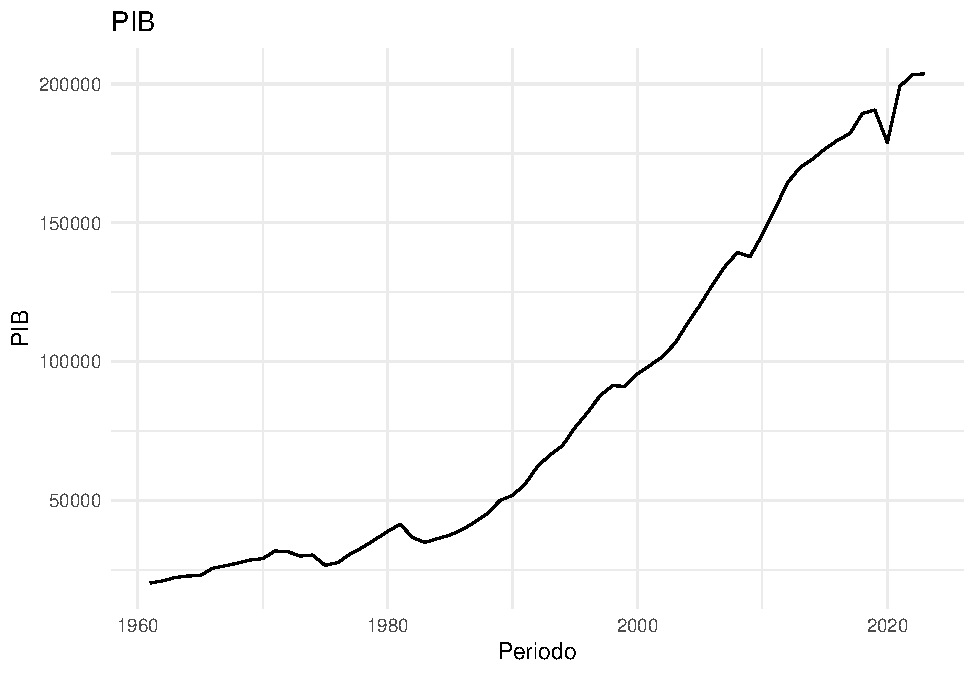
\includegraphics{Ejercicio-4_files/figure-latex/unnamed-chunk-3-1.pdf}

\begin{Shaded}
\begin{Highlighting}[]
\FunctionTok{ggplot}\NormalTok{(base, }\FunctionTok{aes}\NormalTok{(}\AttributeTok{x =}\NormalTok{ Periodo)) }\SpecialCharTok{+}
  \FunctionTok{geom\_line}\NormalTok{(}\FunctionTok{aes}\NormalTok{(}\AttributeTok{y =}\NormalTok{ d\_log\_PIB), }\AttributeTok{color =} \StringTok{"hotpink"}\NormalTok{) }\SpecialCharTok{+}
  \FunctionTok{labs}\NormalTok{(}\AttributeTok{title =} \StringTok{"Dif log del PIB"}\NormalTok{, }\AttributeTok{x =} \StringTok{"Periodo"}\NormalTok{, }\AttributeTok{y =} \StringTok{"Dif log(PIB)"}\NormalTok{) }\SpecialCharTok{+}
  \FunctionTok{theme\_classic}\NormalTok{()}
\end{Highlighting}
\end{Shaded}

\begin{verbatim}
## Warning: Removed 1 row containing missing values or values outside the scale range
## (`geom_line()`).
\end{verbatim}

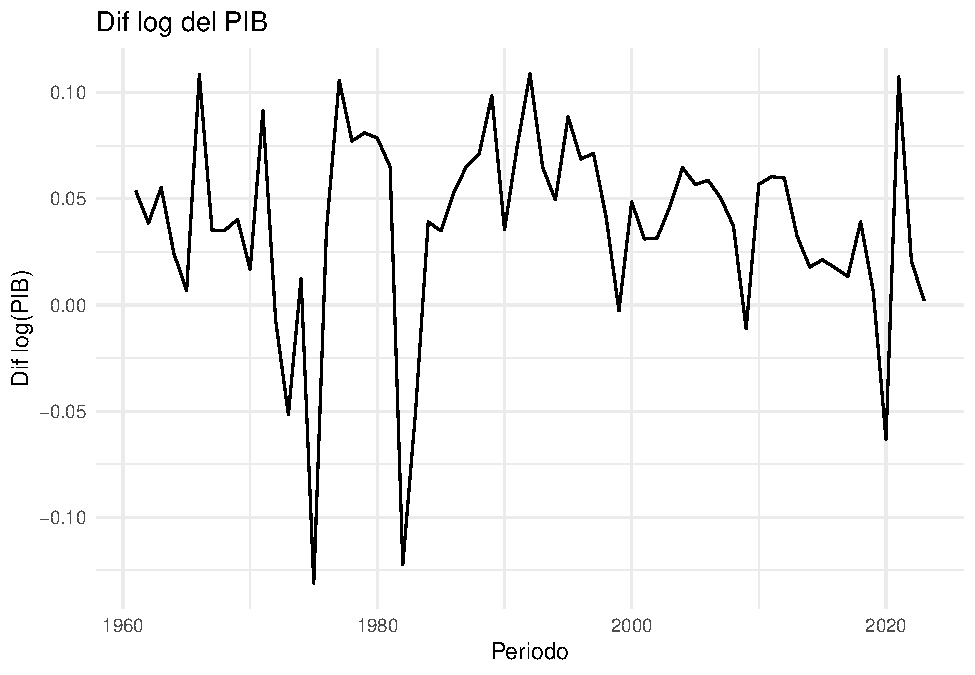
\includegraphics{Ejercicio-4_files/figure-latex/unnamed-chunk-4-1.pdf}

\begin{Shaded}
\begin{Highlighting}[]
\FunctionTok{ggplot}\NormalTok{(base, }\FunctionTok{aes}\NormalTok{(}\AttributeTok{x =}\NormalTok{ Periodo)) }\SpecialCharTok{+}
  \FunctionTok{geom\_line}\NormalTok{(}\FunctionTok{aes}\NormalTok{(}\AttributeTok{y =}\NormalTok{ fbcf), }\AttributeTok{color =} \StringTok{"dodgerblue"}\NormalTok{) }\SpecialCharTok{+}
  \FunctionTok{labs}\NormalTok{(}\AttributeTok{title =} \StringTok{"fbcf"}\NormalTok{, }\AttributeTok{x =} \StringTok{"Periodo"}\NormalTok{, }\AttributeTok{y =} \StringTok{"fbcf"}\NormalTok{) }\SpecialCharTok{+}
  \FunctionTok{theme\_classic}\NormalTok{()}
\end{Highlighting}
\end{Shaded}

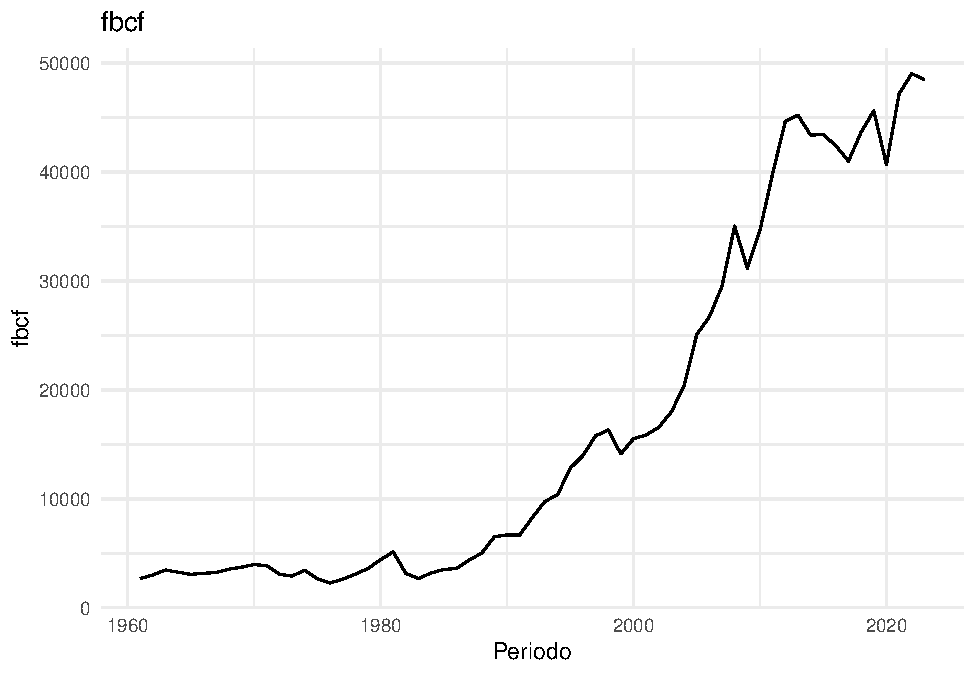
\includegraphics{Ejercicio-4_files/figure-latex/unnamed-chunk-5-1.pdf}

\begin{Shaded}
\begin{Highlighting}[]
\FunctionTok{ggplot}\NormalTok{(base, }\FunctionTok{aes}\NormalTok{(}\AttributeTok{x =}\NormalTok{ Periodo)) }\SpecialCharTok{+}
  \FunctionTok{geom\_line}\NormalTok{(}\FunctionTok{aes}\NormalTok{(}\AttributeTok{y =}\NormalTok{ d\_log\_fbcf), }\AttributeTok{color =} \StringTok{"hotpink"}\NormalTok{) }\SpecialCharTok{+}
  \FunctionTok{labs}\NormalTok{(}\AttributeTok{title =} \StringTok{"Dif log de la fbcf"}\NormalTok{, }\AttributeTok{x =} \StringTok{"Periodo"}\NormalTok{, }\AttributeTok{y =} \StringTok{"Dif log(fbcf)"}\NormalTok{) }\SpecialCharTok{+}
  \FunctionTok{theme\_classic}\NormalTok{()}
\end{Highlighting}
\end{Shaded}

\begin{verbatim}
## Warning: Removed 1 row containing missing values or values outside the scale range
## (`geom_line()`).
\end{verbatim}

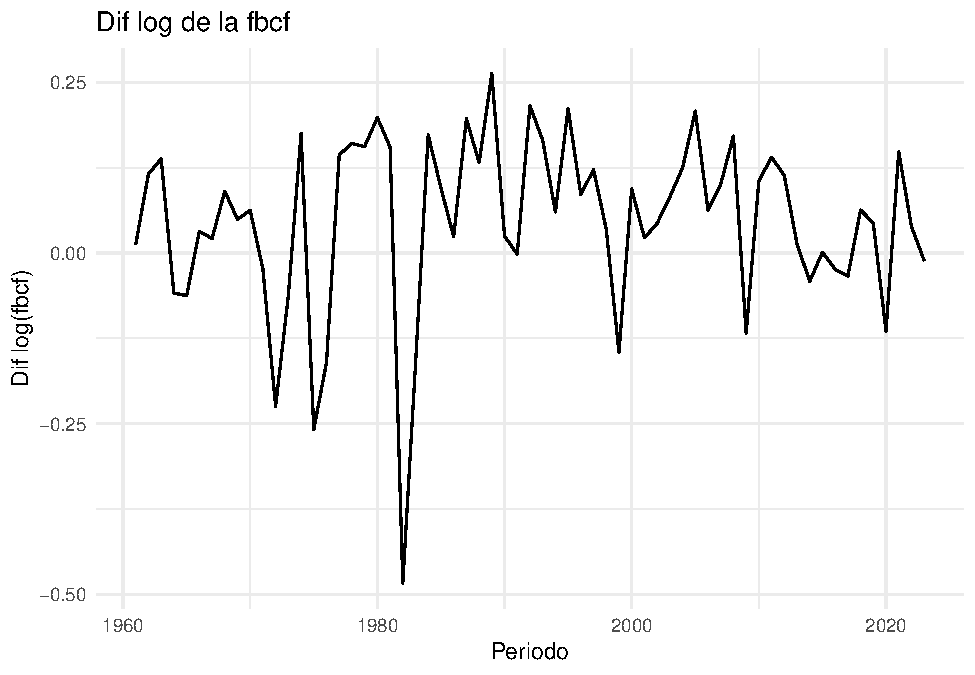
\includegraphics{Ejercicio-4_files/figure-latex/unnamed-chunk-6-1.pdf}

Funciones de Autocorrelación

\begin{Shaded}
\begin{Highlighting}[]
\FunctionTok{acf}\NormalTok{(base}\SpecialCharTok{$}\NormalTok{log\_PIB, }\AttributeTok{main =} \StringTok{"Función de Autocorrelación del log(PIB)"}\NormalTok{)}
\end{Highlighting}
\end{Shaded}

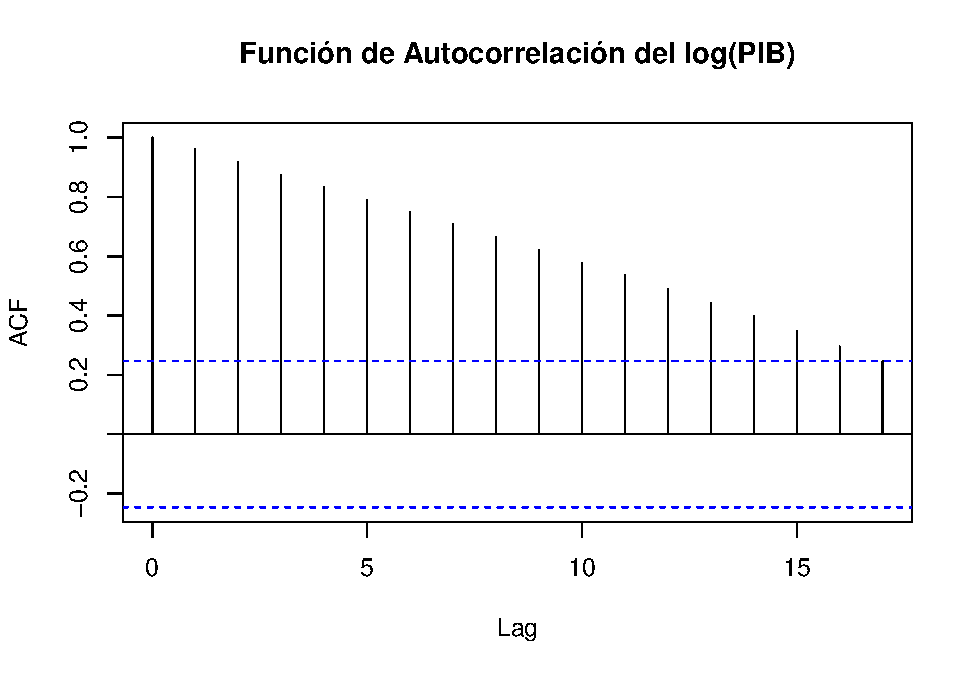
\includegraphics{Ejercicio-4_files/figure-latex/unnamed-chunk-7-1.pdf}

\begin{Shaded}
\begin{Highlighting}[]
\FunctionTok{acf}\NormalTok{(base}\SpecialCharTok{$}\NormalTok{d\_log\_PIB, }\AttributeTok{main =} \StringTok{"Función de Autocorrelación de Dif log(PIB)"}\NormalTok{, }\AttributeTok{na.action =}\NormalTok{ na.pass)}
\end{Highlighting}
\end{Shaded}

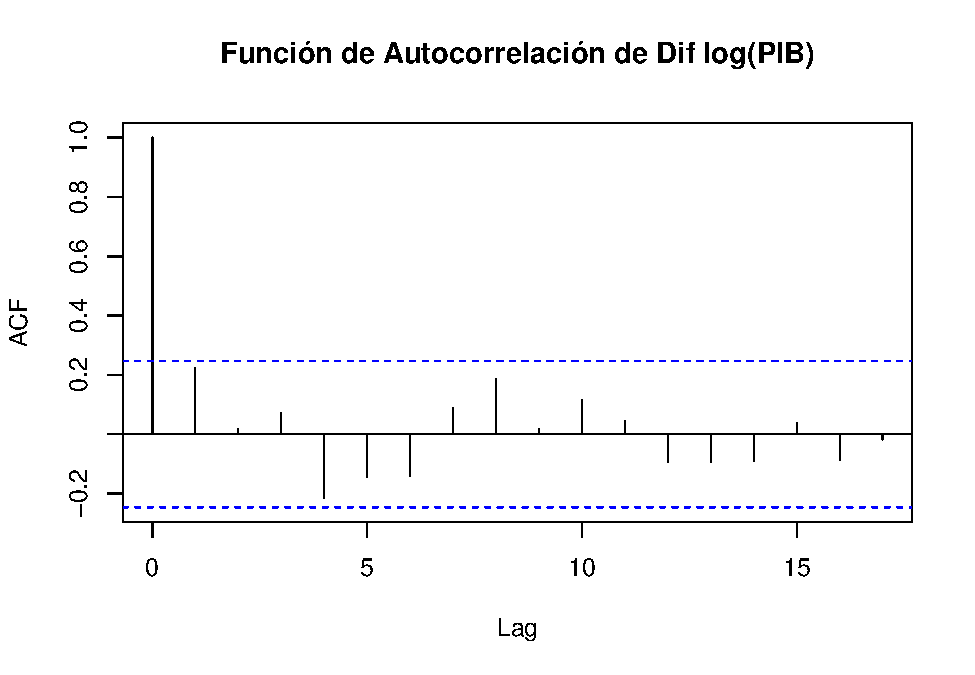
\includegraphics{Ejercicio-4_files/figure-latex/unnamed-chunk-8-1.pdf}

\begin{Shaded}
\begin{Highlighting}[]
\FunctionTok{acf}\NormalTok{(base}\SpecialCharTok{$}\NormalTok{log\_fbcf, }\AttributeTok{main =} \StringTok{"Función de Autocorrelación del log(FBCF)"}\NormalTok{)}
\end{Highlighting}
\end{Shaded}

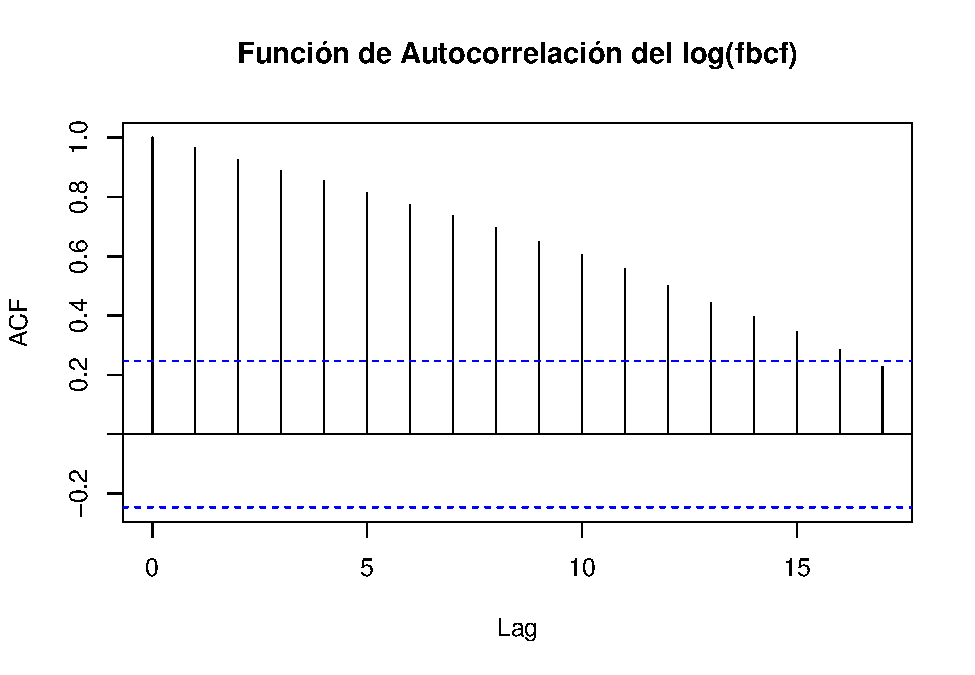
\includegraphics{Ejercicio-4_files/figure-latex/unnamed-chunk-9-1.pdf}

\begin{Shaded}
\begin{Highlighting}[]
\FunctionTok{acf}\NormalTok{(base}\SpecialCharTok{$}\NormalTok{d\_log\_fbcf, }\AttributeTok{main =} \StringTok{"Función de Autocorrelación de Dif log(FBCF)"}\NormalTok{, }\AttributeTok{na.action =}\NormalTok{ na.pass)}
\end{Highlighting}
\end{Shaded}

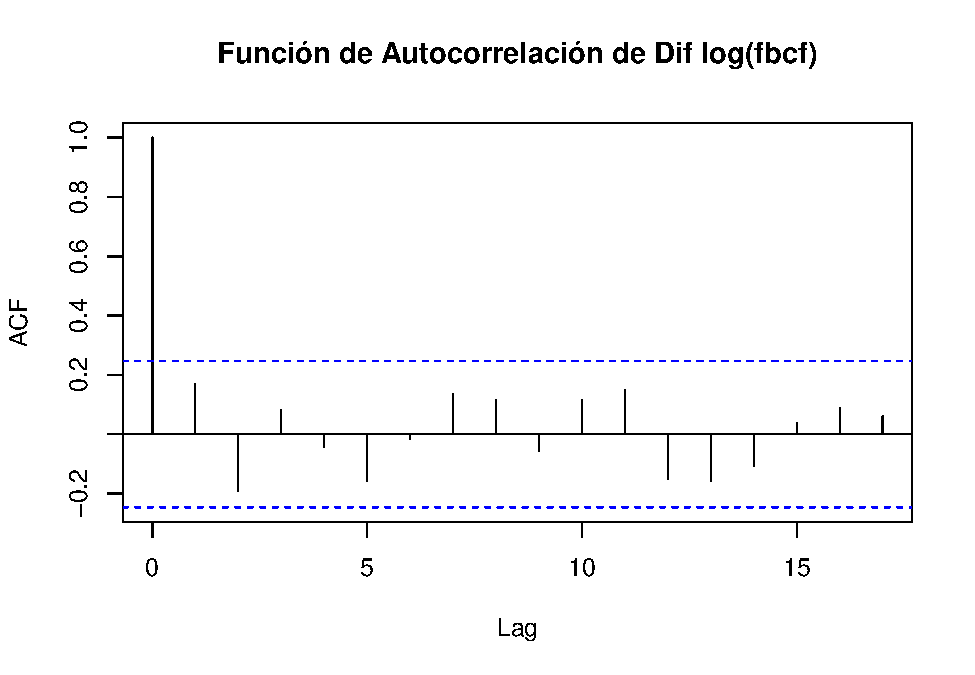
\includegraphics{Ejercicio-4_files/figure-latex/unnamed-chunk-10-1.pdf}

\section{\texorpdfstring{\textbf{\emph{Pregunta
2:}}}{Pregunta 2:}}\label{pregunta-2}

\end{document}
